% Aldono al Dua Libro ("Supplement to the Second Book")
%
% L. L. ZAMENHOF, 1888
%
% XeLaTeX version by Shawn C. Knight, 2019
% XeLaTeX-a versio de Shawn C. KNIGHT, 2019
%
% This work is licensed under a Creative Commons 
% Attribution-NonCommercial-ShareAlike 4.0 International License.
% The original work by Dr. Zamenhof is in the public domain.
%
% Ĉi tiu verko estas permesita per Creative Commons 
% Attribution-NonCommercial-ShareAlike 4.0 Internacia Permesilo.
% La originala verko de D-ro Zamenhof estas senkopirajta.
%
\documentclass[12pt,twoside]{book}

% Version number
%
\newcommand{\laversio}{0.9}

%
% Komuna Enkonduko por Esperantaj Libroj
%

%%%%%%%%%%%%%%%%%%%%%%%%%%%%%%%%%%%%%%%%%%%%%%%%%%%%%%%%%%%%

%
% Geometrio
%
\usepackage[a5paper,margin=2cm]{geometry}

%%%%%%%%%%%%%%%%%%%%%%%%%%%%%%%%%%%%%%%%%%%%%%%%%%%%%%%%%%%%

% 
% Citilojn kaj plu
%
\usepackage[english,french,polish,german,russian,esperanto]{babel}  

%%%%%%%%%%%%%%%%%%%%%%%%%%%%%%%%%%%%%%%%%%%%%%%%%%%%%%%%%%%%

%
% Verso
%
\usepackage{verse}

%%%%%%%%%%%%%%%%%%%%%%%%%%%%%%%%%%%%%%%%%%%%%%%%%%%%%%%%%%%%

%
% Tiparoj
%
\usepackage{fontspec}

% el Google Fonts
\setmainfont{Old Standard TT}
\newfontfamily\cowboyfont{Smokum}[LetterSpace=5]
\newfontfamily\fjallafont{FjallaOne}
\newfontfamily\grammarpartsfont{FjallaOne}[LetterSpace=20]
\newfontfamily\nicefont{Cardo}
\newfontfamily\arbfont{Arbutus Slab}

% en MacOS
\newfontfamily\didone{Didot}
\newfontfamily\copper{Copperplate Light}[LetterSpace=5]
\newfontfamily\chunk{Rockwell}

% el Font Squirrel
\newfontfamily\latinia{Latinia}
\newfontfamily\curve{England Hand DB}

% el dafont
\newfontfamily\monastic{K22 Monastic}
\newfontfamily\bosox{Bosox}

% el dafont kaj ...
\newfontfamily\fr[BoldFont=Fette classic UNZ Fraktur]{UnifrakturMaguntia}

% el Liberation Fonts
\newfontfamily\sansfont{Liberation Sans}[LetterSpace=5]
\newfontfamily\sansfontclose{Liberation Sans}

% en TeXlive
\newfontfamily\csfont{TeX Gyre Schola}
\newfontfamily\bookman{TeX Gyre Bonum}
\newfontfamily\times{TeX Gyre Termes}

% sans-serif bolds in body text
\newcommand\inbold[1]{\scalebox{1}[0.8]{\fjallafont{#1}}}

% Ombroj por ornamoj tiparoj
\usepackage{shadowtext}
\shadowoffset{1pt}

%%%%%%%%%%%%%%%%%%%%%%%%%%%%%%%%%%%%%%%%%%%%%%%%%%%%%%%%%%%%

%
% Pliaj simboloj
%

% Creative Commons ikonoj
\usepackage{ccicons}

% Por ornamoj kiel la "por angloj" etikedo; beletaj sekcilineoj
\usepackage{pgfornament} 

% la xelatex-simbolo en la kompostanta komento
\usepackage{dtk-logos}

% la klasika montra fingro, kiu ekkrius "19a jarcento" se ĝi povus
\usepackage{dingbat}

%
% Substrekoj kaj litera spaco
% 
\usepackage{soul}
\sodef\spaceout{}{.2em}{0.6em}{0pt}
\sodef\spaceoutmed{}{.1em}{0.5em}{0pt}
\newcommand{\narrow}[1]{\scalebox{0.8}[1]{#1}}

% interlinea distanco
\usepackage{setspace} 

% star lines in poems
% 
\newcommand{\pstars}{%
\hspace*{\fill} * \hspace{3em} \raisebox{-1em}{*} \hspace{3em} * \hspace*{\fill}}

% ŝanĝas la grando de la intermorgema signeto por ĝia kunteksto
%
\usepackage{relsize} 

% la krommarĝeno por la unua lineo de ĉiu alineo devus esti kiel la aliaj
%
\usepackage{indentfirst} 

% this will let us make the nice diagonal 1/2 fraction in the prices page
%
\usepackage{units}

% la krommarĝeno por unuobla alineo
%
\usepackage{changepage}

% horitontala formato kaj pluraj kolonoj por la vortaro
%
\usepackage{pdflscape}
\usepackage{multicol}

% granda longa tablo (la "mi ne scias ..." analizo)
%
\usepackage{longtable}

% por la longaj krampoj en la "Mi ne scias" tablo, kaj la vortara
% lineoj de "la" kaj "l'"
%
\usepackage{multirow} 

% titlesec -- better section/chapter headings
%
\usepackage[compact,center]{titlesec}
\titlespacing*{\chapter}{0pt}{6em}{0pt}

% nice section heading for Patro Nia, etc.
%
\newcommand\secthead[3]{%
\vspace{#2}

{\hfil \scalebox{1.6}[1]{\didone{\bf #1}}}

\vspace{#3}}

% fancy page headers, that is, in imitation of the original
%
\usepackage{fancyhdr}
\setlength{\headheight}{15pt}
\pagestyle{fancy}

\fancyhf{}

% remove the rule at top of page
\renewcommand{\headrulewidth}{0pt}

% tabularx helpos meti la Promesoj, kaj difinas la larĝeco de niaj tabloj
% 
% also letters in the alphabet table at end of book
%
\usepackage{tabularx}
\usepackage{array}
\newcolumntype{Y}{>{\centering\arraybackslash}X}
\newcolumntype{+}{>{\global\let\currentrowstyle\relax}}
\newcolumntype{Z}{>{\currentrowstyle}}
\newcommand{\rowstyle}[1]{\gdef\currentrowstyle{#1}%
#1\ignorespaces
}


% this bit removes the page number from the chapter start page
%
\fancypagestyle{plain}{%
  \renewcommand{\headrulewidth}{0pt}%
  \fancyhf{}%
}

% pgfornament line to end a section
%
\newcommand{\sectionline}{
\begin{center}
\pgfornament[width=0.5\textwidth]{89}
\end{center}}

% la "por angloj" etikedo
%
\sodef\angloj{}{.2em}{0.6em}{0pt}
\newcommand{\poranglojbox}{%
\begin{tikzpicture}[every node/.style={inner sep=0pt}]
\node[align=center](Text){\scalebox{1}[1.2]{\didone{\bf\angloj{por Angloj}}}} ;
\node[shift={(5pt,2pt)},anchor=center](CNW) at (Text.north east) {};
\node[shift={(-5pt,2pt)},anchor=center](CNE) at (Text.north west) {};
\node[shift={(-5pt,-2pt)},anchor=center](CSW) at (Text.south west) {};
\node[shift={(5pt,-2pt)},anchor=center](CSE) at (Text.south east) {};
\draw(CNW) to (CNE);
\draw(CSW) to (CSE);
\pgftransformshift{\pgfpoint{-1cm}{-0.537cm}}
\pgftransformscale{0.05};
\pgftransformrotate{90};
\anglojcurlicue{};
\pgftransformreset;
\pgftransformshift{\pgfpoint{1cm}{0.537cm}}
\pgftransformscale{0.05};
\pgftransformrotate{-90};
\anglojcurlicue{};
\end{tikzpicture}}

% the command for the morpheme-separation stroke
%
\renewcommand{\,}{%
{\relsize{-2.5}\raisebox{-1.35ex}{$'$}}}

% kapliteroj por la Vortaro
% 
\newcommand{\vorhead}[1]{\vspace{1.5ex}
{\hfil \scalebox{1.5}[1]{\sansfont{#1}}}
\vspace{1.5ex}}

\newenvironment{outdent}[1]
  {\setlength{\leftskip}{#1}%%
   \setlength{\parindent}{-#1}%%
  }
  {\par}

% Big delimiters in the demo sentence table
%
\newcommand{\tlba}{\scalebox{1}[1.25]\{}
\newcommand{\trba}{\scalebox{1}[1.25]\}}
\newcommand{\tlbb}{\multirow{2}{*}{\scalebox{1}[2.5]\{}}
\newcommand{\trbb}{\multirow{2}{*}{\scalebox{1}[2.5]\}}}
\newcommand{\tlbc}{\multirow{3}{*}{\scalebox{1}[4]\{}}
\newcommand{\trbc}{\multirow{3}{*}{\scalebox{1}[4]\}}}

% Heading for the colophon
%
\newcommand\kolofono{
\fancyhead[C]{}
\titleformat{\chapter}[display]{\centering\sansfont}{\chaptertitlename}{0pt}{\LARGE}
\chapter*{KOMENTO PRI KOMPOSTAĴO.}

\begin{center}
\rule[0.5ex]{0.5\textwidth}{0.4pt}

\emph{Jen versio \laversio{} de ĉi tiu} \XeLaTeX{} \emph{aranĝaĵo.}
\end{center}
}

%
% Dr. Zamenhof's portrait
%
\newcommand\zamenhof{
\thispagestyle{empty}
\begin{center}
 \vspace*{\stretch{1}}
\begin{figure}[!ht]
\centering
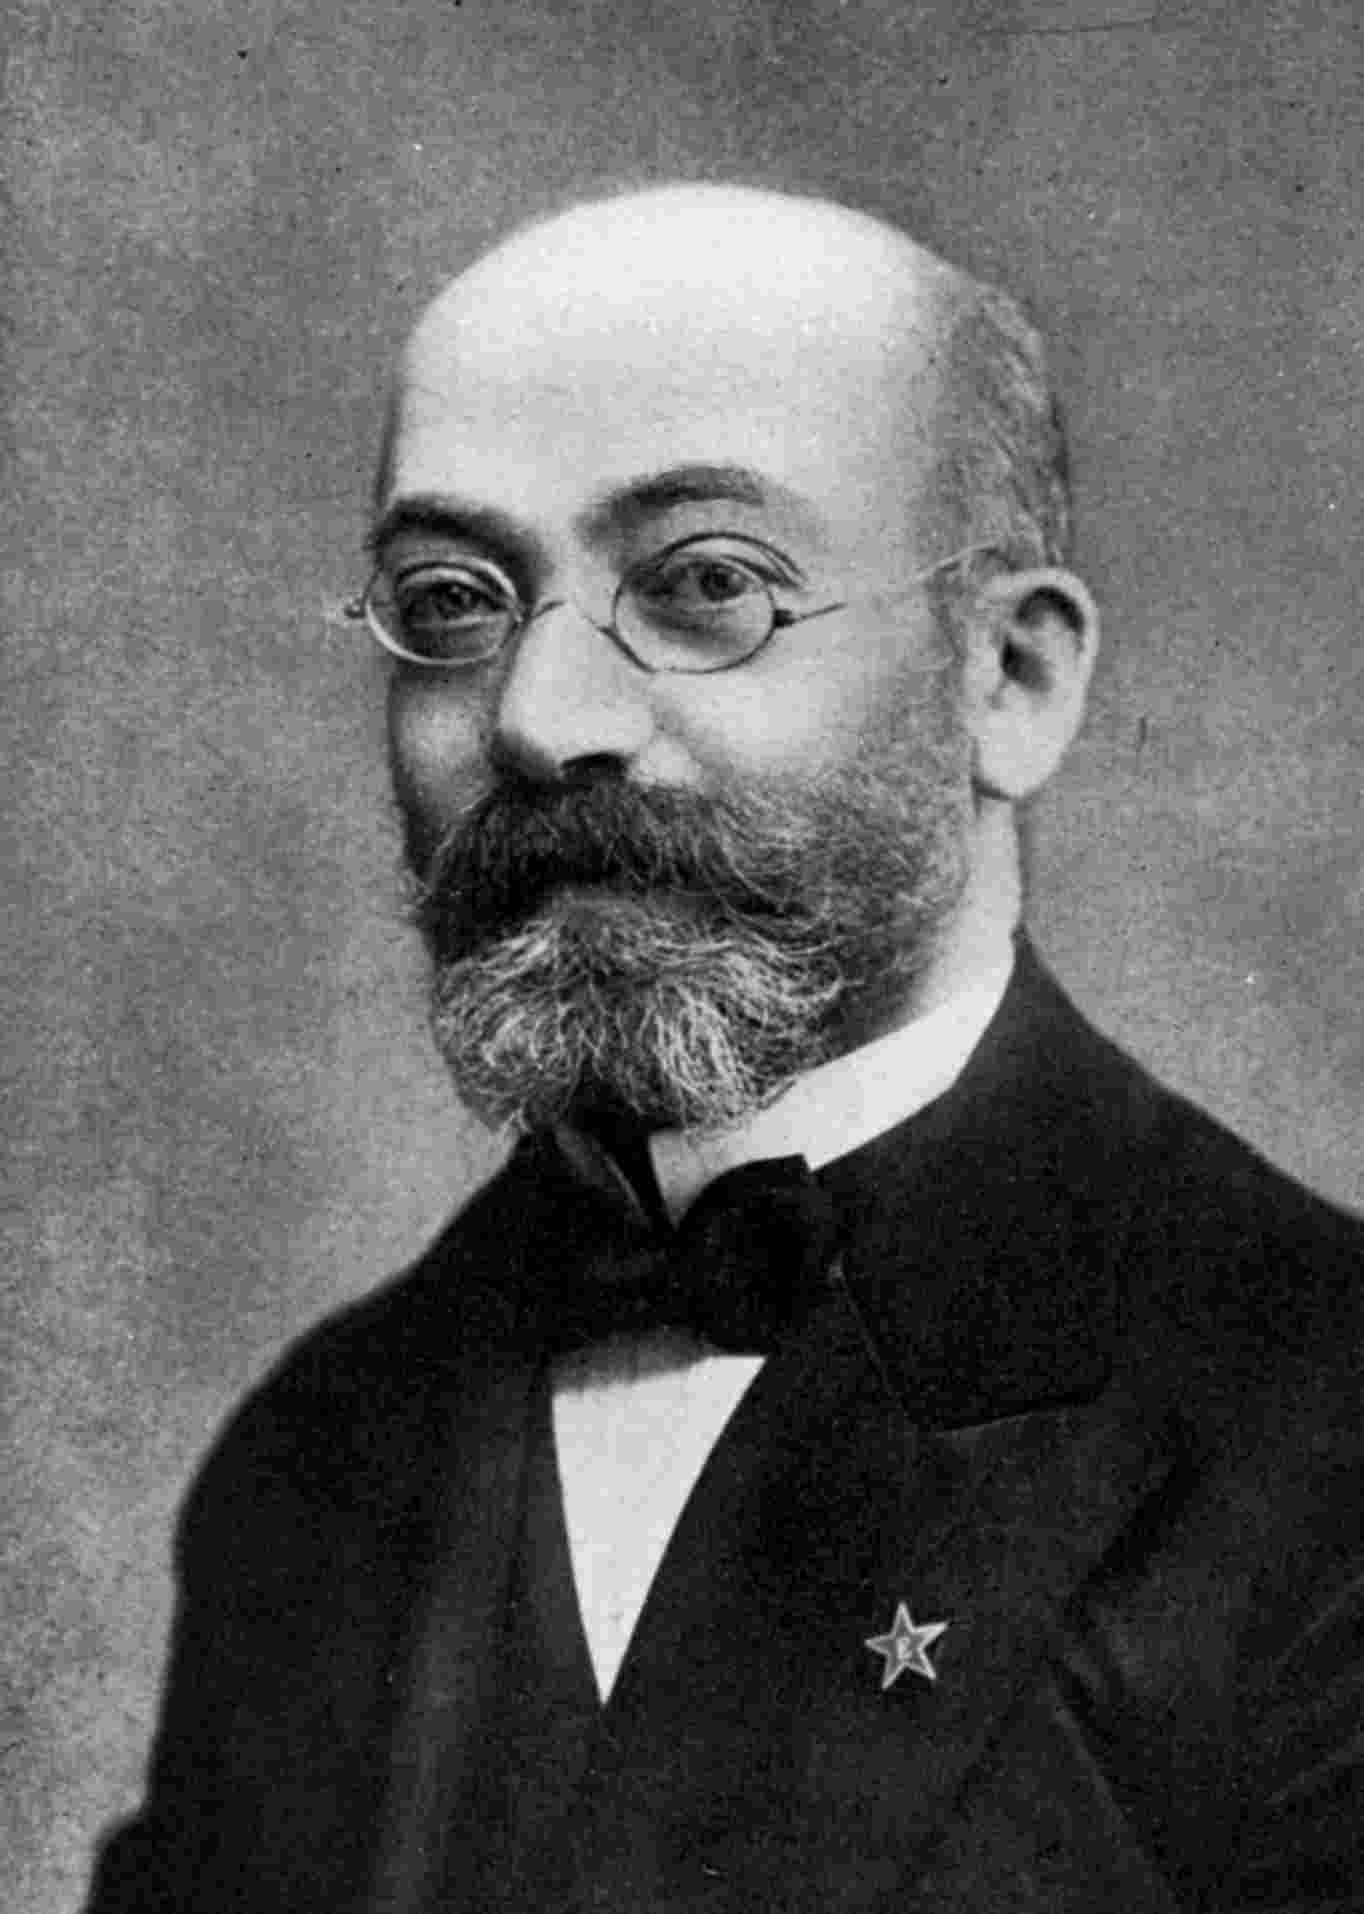
\includegraphics[scale=0.15]{../graphics/Zamenhof}
\end{figure}
\vspace*{0.5cm}
\nicefont
{\LARGE Lazaro Ludoviko ZAMENHOF} \\[1ex]
{\large Aŭtoro de la lingvo «Esperanto»} \\[1ex]
{\small (la 15-a de Decembro 1859 --- la 14-a de Aprilo 1917)}
 \vspace*{\stretch{1}}
\end{center}
\newpage
}

% Ligiloj, kaj ilia koloro 
%
\usepackage{color}
\definecolor{verda_ligilo}{rgb}{0,0.5,0}
\usepackage[colorlinks,linkcolor=verda_ligilo]{hyperref}
\usepackage{bookmark}

%
% Enkonduko speciala por Aldono al Dua Libro
%

% need German-style quotes
% 
\usepackage{csquotes}
\MakeOuterQuote{"}
\setquotestyle{german}

% the command for the morpheme-separation stroke
%
\renewcommand{\,}{\raisebox{-1.1ex}{\relsize{-0.5}{\textquotesingle}}}

\usepackage{nicefrac}

\newcommand\eg{\texttt{=}}

% long side blurbs for the Nomaro table
%
\newcommand\minitab[2]{\begin{tabular}{c}#1 \\ #2\end{tabular}}

\newcommand{\lbOne}{\minitab{10 kopek\,o\,j (Rus.) \eg 12 krejcer\,o\,j (Austr.-Ung.) \eg 20 pfenig\,o\,j (Germ.) \eg}%
{\eg 25 centim\,o\,j (Franc.) \eg 2 \nicefrac{1}{2} penc\,o\,j (Angl.) \eg 5 cent\,o\,j (Amer.)}}

\newcommand{\lbTwo}{\minitab{Anstataŭ mon\,o oni pov\,as send\,i sign\,o\,j\,n de poŝt\,o (de ĉia land\,o).  Por la poŝt\,a}%
{trans\,send\,o oni dev\,as al\,don\,i 10 kopek\,o\,j\,n, egal\,e por paket\,o\,j grand\,a\,j kaj mal\,grand\,a\j.}}

\newlength{\kosto}
\setlength{\kosto}{70pt}


% End preamble and then begin the document
% 
\begin{document}
\sloppy
\setstretch{1.1}

%
% Introduction
%
\titleformat{\chapter}[display]{\centering}{\chaptertitlename}{0pt}{\Huge}
\renewcommand{\footrulewidth}{0pt}
\chapter*{\scalebox{0.8}[1]{ALDONO AL LA}}
\fancyhead[C]{--- \thepage{} ---}

\begin{center}
\vspace{1ex}
\scalebox{1}[1]{\shadowtext{\fjallafont{\LARGE \glqq{}Dua Libro de l’ Lingvo Internacia.\grqq{}}}}

\pgfornament[width=0.3\textwidth]{83}
\end{center}

 En mia unua libro mi petis ĉiujn amikojn de l' lingvo internacia esprimi ilian juĝon pri la lingvo, kiun mi proponis, montri al mi ĉiujn erarojn, kiujn ili trovis en ĝi, kaj ĉiujn plibonigojn, kiujn ili povas proponi, kaj helpi min tiel doni al la lingvo la plej bonan formon, ĉar la finan formon mi intencis doni al la "Lingvo Internacia" ne pli frue ol en la fino de l' jaro 1888, pripensinte kaj provinte antaŭe ĉiujn juĝojn kaj proponojn, kiuj estus senditaj al mi ĝis tiu tempo. En la "Dua Libro" mi diris, ke por fari la lingvon libera de ĉiuj personaj eraroj, estus dezirata, ke ia instruita societo prenu en siajn manojn la sorton de l' lingvo kaj, aŭskultinte la konsilojn de kompetentaj personoj, ĝi donu al la lingvo la finan formon, kiu estus egale ordona por mi, kiel por ĉiu alia amiko de l' lingvo internacia.

Nun mi kun la plej granda ĝojo povas sciigi ĉiujn amikojn de l' lingvo internacia, ke mia deziro ne restis vana. Ankoraŭ en la fino de l' jaro 1887, t. e. ankoraŭ antaŭ la ricevo de mia libreto, la Amerika Filozofia Societo en Filadelfio (The American Philosophical Society) elektis komitaton por pripensi kaj decidi la demandon, ĉu lingvo internacia estas necesa, ĉu ĝi estas kreebla, kaj \emph{kiel} ĝi devas esti. La frukto de l' laboroj de la komitato estis jena decido:

    ke lingvo internacia estas kreebla, ke ĝi estas necesa, ke ĝi devas havi gramatikon la plej simplan kaj naturan, kun la plej simpla ortografio, kaj fonologio, kaj la vortoj devas esti agrablaj por la orelo; ke la vortaro devas esti kreita el vortoj pli malpli rekoneblaj por la plej gravaj civilizitaj popoloj; ke la fina formo de tia lingvo devas esti la frukto de l' laboroj ne de unu persono, sed de la tuta instruita mondo. 

Sur la fondo de ĉio supre dirita, la "Amerika Filozofia Societo" decidis dissendi al ĉiuj instruitaj societoj la proponon fari internacian kongreson de instruituloj por decidi la finan formon de lingvo tutmonda.

Tiel la leganto vidas, ke ne sciante ankoraŭ pri mia laboro, la "Amerika Filozofia Societo" venis al tiuj samaj decidoj pri lingvo tutmonda, al kiuj mi venis, kaj ke la principoj, kiujn la "Amer. Fil. Societo" ellaboris por la lingvo teorie, estas pli malpli egalaj al tiuj, kiujn mi efektivigis praktike. Tial ĝi estas tute natura, ke ricevinte mian libreton jam en la fino de siaj laboroj, la komitato trovis, ke mia lingvo estas sufiĉe proksima al la idealo, kiun ĝi ellaboris teorie. Jen kion diras pri la "Lingvo internacia" sinjoro Henry Phillips, Jr (unu el la tri personoj, el kiuj estis farita la komitato por decidi la demandon pri lingvo tutmonda):

    "La plej nova propono al la publiko kaj ĝis nun la plej simpla kaj la plej racionala, estas la \glqq{}Lingvo internacia,\grqq{} kreita de d-ro S* el Varsovio. La principoj, sur kiuj ĝi estas fondita, estas en la tuto maleraraj; ĝia vortaro ne estas kreita laŭ la persona volo kaj juĝo de l' aŭtoro, sed prenita el la lingvoj franca, germana kaj angla kaj en parto el la latina, kaj ĝi enhavas la vortojn, kiuj estas similaj en tiuj lingvoj; estas faritaj kelkaj ŝanĝoj pro la bonsoneco. Pro tio kaj pro ĝia gramatiko la lingvo estas mirinde facila por lerni, prezentante neniajn el la kalejdoskopaj rompaĵoj kaj ŝiraĵoj de la Volapük'. La gramatiko de tiu lingvo estas el la plej simplaj, tiel simpla, kiel en nia propra lingvo, kaj la reguloj por la kreado de vortoj estas tiel klaraj kaj tiel facilaj, ke la vortaro el radikvortoj povas esti farita tre malgranda \ldots{}" 

Rakontinte mallonge la tutan konstruon de l' "Lingvo internacia" kaj ĝian gramatikon, kaj montrinte kelkajn punktojn, kiuj laŭ lia juĝo devus esti ŝanĝitaj, sinjoro H. Ph. finas:

    "D\textsuperscript{\underline{ro}} S*, kiu skribas sub la nomo de d-ro Esperanto, estas tre modesta en siaj postuloj kaj proponas sian lingvon al la publika kritiko tra la tempo de unu jaro, antaŭ ol li donos al ĝi la finan formon. Post tiu fina trarigardo kaj ŝanĝo li volas prezenti ĝin por la publika uzado. Li petas siajn legantojn promesi lerni la lingvon nur tiam, se 10,000,000 personoj estos donintaj tian saman promeson. Mi esperas, ke la fina trarigardo de l' \glqq{}Lingvo internacia\grqq{} kondukos al la bonigo de l' eraroj, kiujn mi montris, \emph{kaj la tuta mondo povas kuraĝe doni la petitan promeson}". 

La kvar ŝanĝoj, kiujn proponas sinjoro H. Ph., estas \emph{teorie} tre bonaj, sed mi jam mem antaŭ kelkaj jaroj pensis pri ili kaj mi trovis, ke \emph{praktike} ili estus tre maloportunaj. Pli vastan mian juĝon pri ili kaj pri ĉiuj proponitaj ŝanĝoj mi prezentos al la kongreso, se tiu ĉi efektiviĝos. Al ĉiuj ŝanĝoj, kiujn la internacia kongreso de instruituloj post fonda provado trovos necesaj,—mi jam antaŭe donas mian plenan konsenton.

Sciigante la amikojn de l' lingvo internacia pri la intencita internacia kongreso, mi devas sciigi ilin, ke la tuta sorto de l' lingvo internacia de nun transiras en la manojn de l' kongreso, kaj la fina formo, kiun la kongreso donos al la lingvo, devas esti leĝdonanta por ĉiuj amikoj de l' "Lingvo internacia", \emph{se la kongreso eĉ trovus necesa ŝanĝi la lingvon ĝis nerekonebleco.} Mia rolo nun estas finita, kaj mia persono tute foriras de l' sceno.

Sed kunligi jam antaŭe la sorton de l' lingvo internacia kun la estonta kongreso—estus tre malprudenta, kaj tiuj amikoj de l' lingvo, kiuj malfortigus aŭ tute ĉesigus ilian laboradon, "atendante la kongreson,"—povus meti nian sanktan aferon en danĝeron esti perdita je eterne; ĉar la kongreso povas ankoraŭ ne efektiviĝi, kaj se ĝi efektiviĝos, povas ankoraŭ okazi, ke ĝi donos neniajn praktikajn rezultatojn. Tial ni devas labori diligente \emph{laŭ la vojo, kiun ni jam unu fojon elektis,} tute egale ĉu la kongreso efektiviĝos aŭ ne, ĉar \emph{tiu} vojo estas certa kaj kondukos nin al la celo \emph{en ĉiu okazo.} Esperante la kongreson, mi nun faras persone neniajn ŝanĝojn en la lingvo. Ĉiujn ŝanĝojn, kiujn oni proponis al mi, kaj mian personan juĝon pri ili—mi prezentos nun jam ne al la publiko, sed al la estonta kongreso. La eldonado de la ceteraj kajeroj de la "Dua Libro" nun jam tial ne estas bezona, la nuna kajero estas la lasta, kaj la \emph{aŭtoro} nun ĉesigas je eterne sian laboradon. Ĉion, kion mi de nun faros aŭ skribos, mi ĝin ĉion faros jam kiel simpla privata amiko de la lingvo internacia havante nek pli da kompetenteco, nek pli da moralaj aŭ materialaj privilegioj, ol ĉiu alia.

Sed por ke la lingvo internacia povu fariĝi de nun tute sendependa de mia persono, kaj ke ĝi povu tute bone kaj regule riĉiĝi, vastiĝi kaj iri antaŭen, ĉu mi povos ankoraŭ labori por ĝi, aŭ ne,—mi donos tie, unu fojon por ĉiam, respondojn je kelkaj demandoj tuŝantaj la lingvon kaj ĝian estontecon.

1) La lingvo internacia restas senŝanĝa en tiu formo, en kiu ĝi estas proponita de mi; fari en ĝi iajn laŭvolajn ŝanĝojn mi de nun jam ne havas la privilegion; tiu ĉi privilegio apartenas al la internacia kongreso de instruituloj, kiu estas esperata pro la iniciativo de la Amerika Filozofia Societo; se la intencita kongreso ne efektiviĝos, tiam poste (sed ne antaŭ kvin jaroj de nun) la amikoj de l' lingvo internacia faros mem internacian kongreson, kiu havos la privilegion fari en la lingvo ŝanĝojn kaj bonigojn.

2) La sola ŝanĝo, kiun mi trovas necesa fari mem, estas: anstataŭ "ian," "ĉian," "kian," "nenian," "tian"—devas esti: "iam," "ĉiam," "kiam," "neniam," "tiam" (por malegaligi la vortojn "ian" etc. kaj "ia\,n" etc).

3) Se ia el la tipografioj ne povas presi verkojn kun signetoj superliteraj (\^{}) kaj (˘), ĝi povas anstataŭigi la signeton (\^{}) per la litero "h" kaj la signeton (˘) tute ne uzadi. Sed en la komenco de tia verko devas esti presita: "ch \texttt{=} ĉ; gh \texttt{=} ĝ; hh \texttt{=} ĥ; jh \texttt{=} ĵ; sh \texttt{=} ŝ". Se oni bezonas presi ion kun signetoj internaj (\,), oni devas ĝin fari garde, ke la leganto ne prenu ilin por komoj (,). Anstataŭ la signeto (\,) oni povas ankaŭ presadi ({\relsize{-0.5}{\textquotesingle}}) aŭ (-). Ekzemple: sign\,et\,o = sign{\relsize{-0.5}{\textquotesingle}}et{\relsize{-0.5}{\textquotesingle}}o = sig-net-o.

4) La vortaro, kiu estas aldonita al mia unua broŝuro, estas ne plena, kaj la leganto ne miru, se li multajn vortojn en ĝi ne trovas. Sed mi ne havis la intencon eldoni \emph{aŭtore} plenan vortaron kaj krei laŭ mia persona plaĉo la tutan lingvon de l' kapo ĝis la piedoj. Ĉar unue—la kreado de tute plena vortaro estas laboro ne ebla por unu homo, ĉar la nombro de l' vortoj en lingvo de l' homoj estas senfina, kaj se kun ĉiu vorto oni devus atendi, ĝis mi ĝin kreos, tiam la lingvo neniam estus finita kaj ĉiam estus en dependo de mia persono; due—en tia grava afero, kiel lingvo tutmonda, la persona juĝo kaj decidoj de unu homo devas havi rolon eble plej malgrandan, ĉar unu homo sur ĉiu paŝo eraras. Unu homo tie povas esti nur iniciatoro sed ne kreanto. Lingvo tutmonda devas esti pretigata paŝo post paŝo, per la kunigita laborado de la tuta civilizita mondo. Por ke la lingvo povu regule, unuforme kaj unuvoje progresadi malgraŭ la disĵetita laboro de malsamaj personoj en malsamaj lokoj de la tuta mondo, oni devis krei komunan fundamenton, sur kiu ĉiuj povus labori. Tia komuna fundamento por la "Lingvo internacia" devas esti mia unua broŝuro ("Lingvo internacia. Antaŭparolo kaj plena lernolibro"), kiu havas en si la tutan gramatikon de la lingvo kaj sufiĉe grandan nombron da vortoj. Tio ĉi estas la unua kaj la lasta \emph{persona} vorto en la afero de l' lingvo internacia. Ĉio cetera devas esti kreata de la homa societo kaj de la vivo, tiel kiel ni vidas en ĉiu el la vivantaj lingvoj. Ĉiu, kiu ellernis la diritan "fundamenton", povas kuraĝe diri, ke li konas la lingvon internacian tute, ke li konas ĝin ne malpli bone ol la aŭtoro aŭ ol iu alia. Ĉar en ĉio, kio en la dirita broŝuro ne estas trovata, kompetenta devas esti de nun ne la aŭtoro aŭ ia alia persono,—la solaj kompetentaj nun devas esti talento, logiko, kaj la leĝoj kreitaj de la \emph{plej granda parto} de la verkantoj kaj parolantoj.

\emph{Se ia vorto ne estas trovata en la vortaro, kiun mi eldonis, kaj oni ĝin ne povas fari mem laŭ la reguloj de la internacia vortfarado, nek anstataŭigi per alia esprimo,—tiam ĉiu povas krei tiun vorton laŭ lia persona plaĉo;} tiel ankaŭ se naskiĝus ia demando stilistika aŭ eĉ gramatika, ne decidita klare en mia unua broŝuro,—ĉiu povas ĝin decidi laŭ sia juĝo; kaj se vi volas scii, ĉu vi bone decidis tiun demandon, turnu vin ne al mi, sed rigardu, kiel tiun demandon decidas la \emph{plejmulto} de l' verkantoj. \emph{Ĉiu vorto, ĉiu formo, kiu ne estas rekte kontraŭ la jam kreita gramatiko kaj vortaro, aŭ kontraŭ la logiko aŭ la leĝoj enkondukitaj de la plejmulto de l' uzantoj,—estas tute bona,} tute egale ĉu ĝi plaĉos al mi persone aŭ ne. La verkoj, kiujn mi eldonos persone, ne devas havi pli da kompetenteco, ol la verkoj de ĉiu alia. Kaj poste, kiam la lingvo sufiĉe fortiĝos kaj ĝia literaturo sufiĉe vastiĝos, tiam ankaŭ tio, kio estas en mia unua broŝuro, devos perdi ĉian signifon, kaj sole kompetentaj tiam devos esti la leĝoj ellaboritaj de la plejmulto. Per unu vorto—la lingvo internacia devas vivi, kreski kaj progresi laŭ la samaj leĝoj, laŭ kiaj estis ellaborataj ĉiuj vivaj lingvoj, kaj tiu formo, kiun mi donis al ĝi, tiu gramatiko kaj vortaro, kiujn mi prezentis, devas esti sole fundamento, sur kiu estos ellaborata la efektiva lingvo internacia de l' estonteco.

Se mi senigas min nun je ĉiaj personaj privilegioj, kaj fordonas ilin tute al la publiko, mi ĝin faras ne pro malvera modesteco, sed ĉar mi havas la profundan kredon, ke tion postulas la interesoj de la afero, kiu alie ne povus regule kaj rapide vastiĝi kaj ĉiam estus en dependo de unu persono kun liaj eraroj. Nur viva konkursa laboro, ĉe kia ĉio pli bona iom post iom elpuŝas la malpli bonan,—povas doni efektive bonan kaj vivipovantan lingvon internacian.

Multaj kredeble timos, ke danke tiun vastan liberecon la lingvo internacia baldaŭ disfalos en multaj malsamaj lingvoj. Sed kiu konas iom la historion de la lingvoj, tiu komprenos, ke tiu timo estas tute senfonda, ĉar ni ĉiuj laboros sur unu fundamento, kaj tiu fundamento, enhavante la tutan gramatikon kaj la pli grandan parton de l' vortoj, kiuj en la parolado estas renkontataj la plej ofte, havos en la lingvo internacia tian saman signifon, kiun en ĉiu lingvo havis tiu lingva materialo, kiu estis en ĝi en la komenco de regula skriba literaturo: estis preta gramatiko, estis granda kolekto da vortoj, sed multaj vortoj ankoraŭ malestis. Tiuj ĉi vortoj estis kreataj unu post unu, laŭ la kreskanta bezono, kaj malgraŭ ke ili estis kreataj dise de malsamaj personoj, sen ia kondukanto aŭ leĝdonanto, la lingvo ne sole ne disdividiĝis, sed kontraŭe, ĝi ĉiam pli unuformiĝis, la dialektoj kaj provincialismoj iom post iom perdiĝis antaŭ la fortiĝanta komuna literatura lingvo. Ke mia unua broŝuro prezentas fundamenton sufiĉe fortan, kaj ke la fundamenta vortaro enhavas nombron da vortoj sufiĉan kaj tiel grandan, ke se oni volas, oni povas eĉ tute libere esprimi siajn pensojn sen ia kreado de novaj vortoj,—montras la fakto, ke en la tuta "Dua Libro" vi ne renkontas eĉ unu nove kreitan vorton! (vi renkontos tie, vere, multajn vortojn, kiujn vi ne trovas en la fundamenta vortaro, sed tio ĉi estas vortoj ne nove kreitaj, sed nur tiaj, kiujn mi danke la gramatikon (C. 7.) ne bezonis presi en la vortaro). Oni devas memori, ke ĉiu lingvo servas por esprimi niajn pensojn, sed ne por senpense traduki el aliaj lingvoj; oni devas tial peni esprimadi siajn pensojn per la jam estantaj vortoj kaj kreadi novajn vortojn nur tie, kie ĝi estas efektive necesa,—kaj tiam la vortoj nove kreataj estos nur malofte disĵetitaj inter la multo da vortoj jam konataj kaj povos facile aliĝi al la lingvo kaj riĉigi ĝin ne perdigante ĝian unuformecon.

Tiel, danke la unu gramatikon kaj la unu formon de la plej granda parto de l' vortoj, la lingvo internacia havos jam de l' komenco unu formon ĉe ĉiuj uzantaj ĝin. Nur tiuj vortoj, kiuj en la fundamenta vortaro ne estas trovataj, en la unua tempo estos malegale kreataj de malsamaj aŭtoroj. Sed ĉar unue tiaj vortoj estos renkontataj nur disĵetite inter la multo da vortoj jam konstantaj, kaj due la nombro de tiaj malegale sonantaj vortoj ankoraŭ pli malgrandiĝos danke la komunan fonton, el kiu la aŭtoroj prenados la novajn vortojn (la plej gravaj eŭropaj lingvoj),—tial tiuj "novaj" vortoj prezentos nenion alian ol provincialismojn de la unu lingvo internacia. Tiaj provincialismoj estis en granda nombro en ĉia alia lingvo, kaj kun la vastiĝado de la skribata literaturo ili komencis perdiĝi. Tio sama estos ankaŭ en la lingvo internacia, sed ĉar la lingvo internacia pli dependas de la volo de l' homoj, ol de aliaj kondiĉoj,—tiu proceso de unuformiĝado iros en ĝi multe pli rapide. La vortoj kreitaj malfeliĉe baldaŭ perdiĝos, kaj la vortoj feliĉe kreitaj restos kaj eniros en la lingvon; la vortoj egale feliĉe kreitaj sed malegale sonantaj—kelkan tempon batalos inter si kiel sinonimoj, sed jam post mallonga tempo ni vidos, ke unu el tiuj formoj estas uzata pli ofte kaj de pli granda parto de verkantoj, ol ĉiuj aliaj formoj,—kaj baldaŭ la unua formo elpuŝos ĉiujn ceterajn formojn, kiuj post kelka tempo simple mortos de neuzado. Tiel ju pli energie vastiĝos kaj riĉiĝos la literaturo de la lingvo internacia, des pli baldaŭ ni havos unuforman pli malpli plenan vortaron.

Tiuj, kiuj volas labori super la lingvo internacia, skribi verkojn en tiu lingvo etc.—povas nun diri kuraĝe, ke ili havas en la manoj \emph{plenan vortaron}; ĉar povante ĉian ankoraŭ ne kreitan vorton krei laŭ ilia plaĉo, anstataŭ atendi, ĝis \emph{mi} ĝin kreos, ili povas nun esprimi en la lingvo internacia \emph{ĉion}, kion ili volas. Tio ĉi estus ne ebla en la okazo, se mi volus mem eldoni plenajn vortarojn: ĉar kiom ajn mi laborus, ĉiam danke la senfineco de la homa vortaro restus ankoraŭ multego da vortoj ne kreitaj, kaj tiuj, kiuj devus ilin uzi, ne scius kion fari, ĉar krei ilin mem estus ne permesita.

Sed nun restas unu ŝajne tre grava demando: se mi skribas al iu en la lingvo internacia kaj mi devis kelkajn vortojn krei mem, sed mi volas havi la certon, ke la adresito \emph{tute bone, vere kaj klare} komprenos la vortojn, kiujn mi kreis,—kion mi tiam devas fari? La respondo estas tre simpla: fari tion saman, kio estas farata ĉe la uzado de ĉia alia lingvo, se ia por ni necesa vorto en tiu lingvo aŭ tute ankoraŭ ne ekzistas, aŭ ne estas ankoraŭ de ĉiuj egale uzata aŭ konata,—t.~e. \emph{apud la vorto nove kreita meti en kuneteniloj (\ldots{}) la tradukon de tiu vorto en ia alia lingvo, en kiu tiu vorto jam ekzistas.} Kiun lingvon vi uzos por tiu celo, estas por la afero tute egala, se vi nur pensas, ke tiu lingvo estas komprenebla por via adresito, aŭ ke li havas sub la mano aŭ facile povas havi vortaron de tiu lingvo. Sed estus dezirate, ke ĉiuj amikoj de la lingvo internacia uzu en tiaj okazoj unu lingvon, kaj por tio mi proponas la lingvon francan, ĉar tiu ĉi lingvo en nia tempo en multaj sferoj ankoraŭ havas la rolon de lingvo internacia. \emph{Sed tute ne estas postulata, ke vi aŭ via adresito sciu la lingvon francan,} ĉar la vorto devas esti elskribata el la franca vortaro sen ia ŝanĝo, en tiu formo, en kiu ĝi estas trovata en la vortaro; estas nur necese, ke la skribanto kaj la ricevanto havu sub la mano francan vortaron (se ili ne pli volas uzi alian lingvon).

Multaj kredeble estos malkontentaj, ke mi ne volas eldoni persone plenan aŭtoritatan vortaron, kiun ĉiuj devus obei. La amaso amas, ke oni donu al ĝi leĝojn, ke oni donu al ĝi ne bonan, sed jam tute pretan,—kaj la vojon, kiun mi proponas, multaj nomos tro malrapida. Se mi ne eldonas mem vortarojn pli plenajn, sed lasas ilian kreadon al la publiko, mi ĝin faras ne pro maldiligento: sufiĉe plena vortaro jam estas preta ĉe mi, kaj mi povus eldoni ĝin eĉ tuj, kaj se ĝi eĉ ne estus preta, la leganto komprenos, ke ĝi estas tute ne malfacila por mi krei ĉiutage certan nombron da vortoj kaj eldonadi paŝo post paŝo vortarojn ĉiam pli plenajn. Por mi \emph{persone} estus kompreneble multe pli oportuna teni la sorton de l' lingvo internacia en miaj manoj. Tial, mi esperas, la leganto komprenos, ke kreinte la fundamenton de l' lingvo, mi nun deprenas de mi tutan aŭtoritaton nur tial, ke mi profunde kredas, ke tion postulas la interesoj de l' afero. La tempo, mi esperas, montros, ke mi ne eraris. Sed se la estonteco eĉ montros, ke mi eraris kaj ke plena vortaro devas esti kreata de \emph{unu} persono, la leganto ne forgesu ke mi ja povas ĝin fari ankaŭ poste! Sed mi faros ĝin nur tiam, se la tempo montros, ke ĝi estas efektive \emph{necesa}. Nun mi laborados, mi skribados verkojn, mi kreados vortojn,—sed ĉion kiel privata amiko de l' lingvo internacia, kaj ĉiu alia povas ĝin fari kun la egala kompetenteco.

5) Je la demando, kiam mi eldonos vortarojn returnitajn (nacia-internaciajn), kiam mi eldonos mian broŝuron en ĉiuj aliaj lingvoj, ĉu mi eldonos lernolibrojn sistemajn kaj vastajn, librojn, gazetojn etc.—mi jam nun ne bezonas respondi; ĉar, konante nun la lingvon internacian ne malpli ol mi mem, kaj estante nun egala morala kaj materiala mastro de la lingvo kiel mi mem,—ĉiu povas nun mem eldoni ĉiajn necesajn verkojn, ne atendante ĝis mi ĝin faros. Mi faros, kion mi povos, kaj ĉiu alia amiko de l' lingvo faru ankaŭ, kion li povas; mi mem ne povas eldoni eĉ la centan parton de tio, kio estas bezonata.

6) Multaj petas, ke mi komencu eldonadi la adresarojn de la "promesintoj", por ke la amikoj de l' lingvo internacia sciu unu pri alia kaj povu korespondi inter si. Tiujn adresarojn mi kredeble efektive komencos eldonadi, sed nur tiam, kiam mi vidos, ke la homoj efektive komprenis la gravecon de l' promesoj kaj prenas la aferon sufiĉe serioze. Sed nun estas bedaŭrinde ankoraŭ multaj, kiuj, vive laborante por la afero kaj tute bone korespondante en la lingvo internacia, ne sendis ankoraŭ ilian "promeson"!

7) Multaj min demandas, per kio ili povas esti utilaj al la afero de l' lingvo internacia, kiel ili devas labori kaj kiel oni povas la plej certe progresigi la aferon. Mia respondo nun devas esti: ĉiu laboru tiel, kiel li trovos la plej bona, ĉar la sorto de l' afero estas nun egale en la manoj de ni ĉiuj. Celon ni ĉiuj havas unu kaj klaran: ke la nombro de l' amikoj de l' lingvo internacia, la nombro de l' personoj uzantaj tiun lingvon kaj laborantaj por ĝi—konstante kresku, kaj ke la lingvo mem ĉiam pli riĉiĝu. Por tio ni ne bezonas kondukanton: ĉia persono, ĉia rondeto, ĉia societo laboru laŭ sia bontrovo, en sia sfero kaj laŭ siaj fortoj,—kaj malgraŭ la disĵeteco de l' laboro (se ĝi nur estos ĉie sufiĉe energia) post la plej mallonga tempo ni vidos, ke nia komuna celo estas alvenita, ke la lingvo internacia fortiĝis kaj estas uzata de la tuta mondo. Tie ĉi mi nur uzos la bonan okazon kaj esprimos per kelkaj vortoj mian \emph{personan} penson pri tio, kiel ni devas faradi:

\emph{a}) Antaŭ ĉio (kaj tio ĉi estas la plej grava) ni devas labori diligente kaj ne malvarmiĝante por la afero kaj tute ne zorgante tion, kion diras aŭ faras aliaj. Estas multaj, kiuj komprenante bone la utilecon de l' afero, alfalis al ĝi en la komenco tre varmege, certe kredante, ke post kelkaj monatoj la tuta mondo jam estos plena de la lingvo internacia; sed kiam post kelka tempo ili vidis, ke la mondo estas ankoraŭ trankvila, ke la plej granda parto de l' mondo eĉ ankoraŭ ne scias pri la afero, ke la gazetoj ne alportas ĉiutage sensaciajn novaĵojn pri la irado de l' afero,—ili tute malvarmiĝis por la afero. De la efemera laboro de \emph{tiaj} amikoj la afero ne sole nenion gajnas, sed kontraŭe, ĝi nur perdas. Sed \emph{efektivaj} amikoj de l' afero ne rigardas, ĉu la afero jam faris multon da bruo kaj ĉu ĝi estas jam sufiĉe "en modo"; profunde kredante, ke la afero estas utila kaj havas estontecon, ili laboras senbrue, sed diligente kaj konstante, ĉiu en sia urbo, en sia lando kaj laŭ siaj fortoj,—kaj danke la laboron de \emph{tiuj ĉi} amikoj mi esperas, ke l' afero baldaŭ kaj sen bruo vastiĝos en la tuta mondo.

\emph{b}) Oni devas energie kolekti "promesojn", ne timante la altecon de la nombro. Mi ripete turnas la okulojn de l' amikoj sur tiun ĉi punkton, ŝajne fantazian, sed efektive tre gravan. Ĉiu el la promesoj aparte havas signifon tre malgrandan, kaj tial multaj ne volas kolekti, dirante, ke promesojn oni devas sendi en granda nombro aŭ tute ilin ne sendi. Mi ripetas, ke tia parolado estas tute malprava. Ne estimante apartajn unuojn, ni neniam venos al grandaj nombroj. Ĉiu promeso aparte havas signifon la plej malgrandegan, sed unu post unu ilia nombro grandiĝos, kaj tiam ili prezentos grandegan forton kaj decidos per unu fojo la gravan demandon de lingvo internacia. Se miaj vortoj estas ne sufiĉe kredigaj, kaj vi restas skeptikaj, ne forgesu almenaŭ, ke \emph{malutilon} la promesoj en ĉia okazo ne portas, se ili eĉ neniam venos al la esperata nombro, sed \emph{utilon} ili ĉe feliĉaj rezultatoj povas alporti grandegan.

\emph{c}) Grandegan utilon alportos al la afero tiuj, kiuj riĉigos la \emph{literaturon} de l' lingvo internacia. Nenio povas tiel bone imponi al la amaso, kiel faktoj kaj konstantaj \emph{signoj de vivo.} Oni devas senĉese eldonadi ĉiam novajn verkojn pri la lingvo internacia, kaj la plej grava—\emph{en} tiu lingvo. La kampo tie ĉi estas granda, eldoni oni povas kaj devas multe. Antaŭ ĉio la amikoj devas eldoni la gramatikon kaj la vortaron en ĉiuj lingvoj de la mondo. Eldoninte la gramatikon kaj la vortaron en la lingvo de iu popolo, vi ne sole donos al tiu popolo la eblon aliĝi al la homara afero, sed unutempe (danke la vortareton) vi per unu fojo donas al la tuta mondo la eblon korespondi libere kun ĉiu ano de tiu popolo. La eldonado de la malgranda vortareto en ĉia aparta lingvo postulas malmulte da laboro kaj tre malmultege da mono. Oni devas eldoni vortarojn returnitajn; ĉar estas jam eldonitaj vortaroj rektaj, la pretigado de vortaroj returnitaj estas laboro tre facila kaj malmulte kosta. Laŭ la mezuro de la progresado kaj riĉiĝado de l' lingvo oni devas eldonadi pli plenajn vortarojn, kaj estus bone, ke en ili la novaj vortoj, kreitaj de l' aŭtoroj mem, estus donitaj kune kun ilia franca traduko. Oni devas eldoni pli vastajn lernolibrojn, laŭ bonaj metodoj, kun multaj ekzemploj kaj pecoj por traduki,—ĉar la lernolibroj, kiujn mi eldonis mem, estas tre malgrandaj, kunpremitaj kaj faritaj nur por homoj pli-malpli instruitaj. Fine, por ke la lingvo eble pli rapide fortiĝu kaj riĉiĝu, oni devas eldoni kiel eble pli multe da verkoj en la lingvo internacia, originalaj aŭ tradukitaj; kaj tiuj personoj aŭ rondetoj, kiuj havas la eblon, devas komenci eldonadi gazetojn kaj ĵurnalojn en la lingvo internacia.

El ĉiuj specoj de verkoj, pri kiuj mi parolis, mi \emph{mem} povas eldoni nur tre malgrandan parton, ĉar mi havas tro malmulte da tempo kaj tro malgrandajn kapitalojn. Ĉiu el la amikoj de l' lingvo aparte povas ankaŭ eldoni nur malmulte. Sed se ĉiu el ni faros tiun malmulton, kiun li povas, tiam la literaturo de l' lingvo internacia rapide vastiĝos.

Por ke ĉiuj povu scii pri ĉiu nova eldonita verko, mi petas ĉiun, kiu eldonos ion pri la lingvo internacia aŭ en tiu ĉi lingvo, sendi al mi unu ekzemplaron de sia verko; ĉar komencante de Aŭgusto 1888 mi eldonados ĉiumonate nomarojn de ĉiuj verkoj pri la lingvo internacia, kiuj eliris de la komenco ĝis tiu tempo. Apud ĉiu verko estos dirita, kiu ĝin eldonis, kiom ĝi kostas kaj kie oni ĝin povas ricevi. Alsendinte la koston de poŝta transsendo, ĉiu povas en ĉiu tempo ricevi de mi la plej novan nomaron de l' verkoj. \emph{La eldonantojn de l' verkoj mi petas ankaŭ, ke en la fino de ĉia verko aŭ verketo, kiun ili eldonos, ili presu ĉiam la plej novan el la diritaj nomaroj.} Mi esperas, ke neniu el la eldonantoj malkonsentos plenumi mian peton, kiu estas egale grava por la eldonantoj kiel por la afero mem.

\emph{ĉ}) Tre grava por la progresado de l' lingvo internacia estas diligenta uzado ĝin en korespondado kun amikoj kaj konatoj aŭ eĉ kun nekonatoj. Kiom ajn vi ripetados al la amaso pri la utileco kaj la oportuneco de l' lingvo, la plej granda parto de l' amaso restos surda por viaj vortoj, ĉar ĝi timos, ke vi postulas de ĝi ian oferon. Sed se ĉiuj amikoj de l' lingvo internacia anstataŭ paroladi \emph{farados}, tiam vi baldaŭ vidos, ke la tuta indiferenta amaso aliĝis jam al la afero, sen bruo kaj eĉ mem tion ne vidinte. Ricevinte de vi leteron internacian kaj kompreninte ĝin, kvankam li la lingvon ne lernis, via adresito vidos \emph{praktike} la oportunecon de l' lingvo, kaj li komencos mem ĝin uzadi; se li restos indiferenta, tiam ricevinte kelkajn fojojn tiajn leterojn, li jam scios sufiĉe bone la lingvon, tute ĝin ne lerninte.

\emph{d}) Estas kompreneble ankoraŭ multaj vojoj kaj vojetoj por progresigi l' aferon de l' lingvo internacia, sed mi devas ilin lasi al la bontrovo kaj plaĉo de ĉiu aparta persono. Estus bone, se en ĉiuj urboj kaj urbetoj estus kreitaj rondetoj por kune labori por la afero de l' lingvo (en kelkaj urboj tiaj rondetoj jam estas kreitaj). Per pripensado kaj laborado kunligita oni ĉiam povas pli multe fari, ol laborante aparte. Sed unu aferon oni ne devas forgesi: oni devas esti atendemaj kaj konstantaj; ni ne devas atendi, ke aliaj nin kuraĝigu per sia ekzemplo, kaj ni ne devas perdi la kuraĝon kaj malvarmiĝi, se ni tiun ekzemplon ne vidas,—ni devas per nia propra laboro doni ekzemplon al aliaj; kaj se en la unua tempo neniu al ni aliĝos, aŭ se oni eĉ ridos je ni, ni devas kredi, ke pli aŭ malpli frue la ridantoj venos al ni. Ni iru kuraĝe antaŭen, ĉar nia afero estas honesta kaj utila!

\begin{center}
\pgfornament[width=0.3\textwidth]{83}
\end{center}

Tiu ĉi libreto estas la lasta vorto, kiun mi elparolas en rolo de aŭtoro. De tiu ĉi tago la estonteco de l' lingvo internacia ne estas jam pli multe en miaj manoj, ol en la manoj de ĉia alia amiko de la sankta ideo. Ni devas nun ĉiuj egale labori, ĉiu laŭ siaj fortoj. Ĉiu el vi povas nun fari por nia afero tiom same kiom mi, kaj multaj el vi povas fari multe pli multe ol mi, ĉar mi estas sen kapitaloj, kaj el mia tempo, okupita de laboro por ĉiutaga pano, mi povas oferi al la amata afero nur tre malgrandan parton. Mi faris por la afero ĉion, kion mi povis, kaj se ĉiu efektiva amiko de l' lingvo internacia alportos al ĝi eĉ la centan parton de l' moralaj kaj materialaj oferoj, kiujn mi al ĝi alportis tra dekdu jaroj ĝis hodiaŭ, tiam la afero iros bonege kaj venos al la celo post la plej mallonga tempo. Ni laboru kaj esperu!

\begin{center}
\pgfornament[width=0.3\textwidth]{83}
\end{center}

\newgeometry{margin=1cm}
\fancyhf{}
\newpage
\begin{center}
\footnotesize
\begin{tabularx}{\textwidth}{m{3ex}r@{ }p{0.5\textwidth}@{ }b{6em}m{3ex}}

\multirow{18}{*}{%
\rotatebox{90}{\parbox{15cm}{\centering%
10 kopek\,o\,j (Rus.) \texttt{=} 12 krejcer\,o\,j (Austr.-Ung.) \texttt{=} 20 pfenig\,o\,j (Germ.) \texttt{=} \\
\texttt{=} 25 centim\,o\,j (Franc.) \texttt{=} 2 \nicefrac{1}{2} penc\,o\,j (Angl.) \texttt{=} 5 cent\,o\,j (Amer.) }}} &
\multicolumn{3}{p{0.7\textwidth}}{\centering \scalebox{1.6}[1]{\didone{\normalsize \bf NOM\,AR\,O}}} &
\multirow{18}{*}{%
\rotatebox{90}{\parbox{15cm}{\centering%
Anstataŭ mon\,o oni pov\,as send\,i sign\,o\,j\,n de poŝt\,o (de ĉia land\,o).  Por la poŝt\,a \\
trans\,send\,o oni dev\,as al\,don\,i 10 kopek\,o\,j\,n, egal\,e por paket\,o\,j grand\,a\,j kaj mal\,grand\,a\j. }}} \\

& \multicolumn{3}{p{0.7\textwidth}}{\small \centering de l' verk\,o\,j pri la lingv\,o inter\,naci\,a (Esperanta),
kiu\,j el\,ir\,is ĝis Juni\,o 1888.} & \\
& & & \multicolumn{1}{c}{\didone{\textbf{Kosto:}}} & \\

& 1) &
Международный языкъ Преди\-словіе и полный учебникъ. (Lingv\,o inter\,naci\,a. El\,don\,o por \textit{Rus\,o\,j}) \dotfill & 
\parbox[t][2\baselineskip][b]{6em}{15 kopek\,o\,j.} \\

& 2) & 
J\k{e}zyk mi\k{e}dzynarodowy. Przedmowa i podr\k{e}cznik kompletny. (Lingv\,o inter\,\-naci\,a. El\,don\,o por \textit{Pol\,o\,j}) \dotfill &
\parbox[t][2\baselineskip][b]{6em}{15 kopek\,o\,j.} \\

& 3) & 
Langue internationale. Préface et manuel complet. (Lingv\,o inter\,naci\,a. El\,don\,o por \textit{Franc\,o\,j}) \dotfill & 
\parbox[t][2\baselineskip][b]{6em}{50 centim\,o\,j.}\\

& 4) & 
Internationale Sprache. Vor\-rede und voll\-ständiges Lehr\-buch. (Lingv\,o inter\,\-naci\,a. \newline El\,don\,o por \textit{German\,o\,j}) \dotfill &
\parbox[t][2\baselineskip][b]{6em}{40 pfenig\,o\,j.}\\

& 5) & 
International tongue. Preface and complete method. (Lingv\,o inter\,naci\,a. El\,don\,o por \textit{Angl\,o\,j}) \dotfill &
\parbox[t][2\baselineskip][b]{6em}{5 penc\,o\,j.}\\

& 6) & Vort\,ar\,o por Rus\,o\,j \dotfill & 3 kopek\,o\,j. \\
& 7) & Vort\,ar\,o por Pol\,o\,j \dotfill & 3 kopek\,o\,j. \\
& 8) & Vort\,ar\,o por Franc\,o\,j \dotfill & 7 centim\,o\,j. \\
& 9) & Vort\,ar\,o por German\,o\,j \dotfill & 6 pfenig\,o\,j. \\
& 10) & Vort\,ar\,o por Angl\,o\,j \dotfill & 1 penc\,o. \\

& 11) & \didone{\textbf{Du\,a libr\,o de l' lingv\,o inter\,\-na\-ci\,\-a. Kajer\,o Nr. 1.}} \dotfill &
\parbox[t][\baselineskip][b]{6em}{25 kopek\,o\,j.}\\

& 12) & Al\,don\,o al la Du\,a Libr\,o de l' Lingv\,o Inter\,naci\,a \dotfill &
\parbox[t][\baselineskip][b]{6em}{10 kopek\,o\,j.} \\

& \multicolumn{3}{p{0.7\textwidth}}{{\large\HandCuffRight{}} Ĉiu\,j supr\,e skrib\,it\,a\,j verk\,o\,j pov\,as est\,i ricev\,at\,a\,j en ĉia libr\,ej\,o kaj ankaŭ ĉe \sansfontclose{\textit{D-r\,\thinspace{}o L. Zamenhof' en Varsovi\,\thinspace{}o.}}} \\

& \multicolumn{3}{p{0.7\textwidth}}{\centering Adreso: \scalebox{0.9}[1]{\didone{\textbf{Dr. L. Samenhof}}} a \scalebox{0.9}[1]{\didone{\textbf{Varsovie}}} (Rus. Pol.)} \\

\cline{2-4}

& \multicolumn{3}{p{0.7\textwidth}}{\centering Дозволено Цензурою. Варшава, 6 Іюня 1889 г.} \\

\cline{2-4}

& \multicolumn{3}{p{0.7\textwidth}}{\centering \bf Presejo de Ĥ. Kelter, Varsovio, strato Nowolipie N. 11.} \\

\\

\end{tabularx}

\end{center}
\restoregeometry
\titlespacing*{\chapter}{0pt}{0em}{0pt}

% kolofono
%
\kolofono

\vspace{1ex}

{\setlength{\parindent}{0em}
Shawn KNIGHT (angle elparolata \emph{ŝan najt})\\
\hodiau}

\newpage
\thispagestyle{empty}
\vspace*{\fill}
\begin{center}
Ĉi tiu verko estas permesita per Creative Commons \\
Attribution-NonCommercial-ShareAlike 4.0 \\
Internacia Permesilo.

La originala verko de D-ro Zamenhof \\
estas senkopirajta.\\[2ex]

\ccbyncsa\\[2ex]

This work is licensed under a Creative Commons \\
Attribution-NonCommercial-ShareAlike 4.0 \\
International License.

The original work by Dr. Zamenhof \\
is in the public domain.
\vspace*{\fill}
\end{center}
\end{document}